% =====================================================================
%  QuestCash — EP.03.01 / Entregable ED, Semana 3
%  Monitoreo, firewall y balanceador de carga
%  Compilar con:  pdflatex reporte_semana3.tex   (dos veces)
%
%  Continuación directa del reporte de la semana 2 (autenticación JWT):
%  reutiliza su preámbulo, paleta y estilos.
% =====================================================================
\documentclass[11pt,letterpaper]{article}

\usepackage[utf8]{inputenc}
\usepackage[T1]{fontenc}
\usepackage[margin=2.4cm,top=2.8cm,bottom=2.6cm]{geometry}
\usepackage{xcolor}
\usepackage{graphicx}
\usepackage{booktabs}
\usepackage{longtable}
\usepackage{array}
\usepackage{enumitem}
\usepackage{fancyhdr}
\usepackage{titlesec}
\usepackage{caption}
\usepackage{tcolorbox}
\usepackage{listings}
\usepackage{tikz}
\usepackage{amssymb}
\usepackage[hidelinks]{hyperref}

\usetikzlibrary{positioning,arrows.meta,shapes.geometric,calc}
\tcbuselibrary{skins,breakable}

% ---------- Español (sin babel: se renombran los rótulos a mano) ----------
\renewcommand{\tablename}{Tabla}
\renewcommand{\figurename}{Figura}
\renewcommand{\refname}{Referencias}
\renewcommand{\contentsname}{Contenido}

% ---------- Paleta (idéntica a la del reporte de la semana 2) ----------
\definecolor{qcNavy}{HTML}{0F2E4C}
\definecolor{qcBlue}{HTML}{2563EB}
\definecolor{qcGreen}{HTML}{16A34A}
\definecolor{qcRed}{HTML}{DC2626}
\definecolor{qcAmber}{HTML}{B45309}
\definecolor{qcGray}{HTML}{6B7280}
\definecolor{qcLight}{HTML}{F3F4F6}
\definecolor{qcCodeBg}{HTML}{111827}

% ---------- Encabezado / pie ----------
\pagestyle{fancy}
\fancyhf{}
\fancyhead[L]{\footnotesize\color{qcGray}QuestCash · EP.03.01 — Semana 3}
\fancyhead[R]{\footnotesize\color{qcGray}Monitoreo, firewall y balanceo}
\fancyfoot[C]{\footnotesize\color{qcGray}\thepage}
\renewcommand{\headrulewidth}{0.4pt}
\renewcommand{\headrule}{\hbox to\headwidth{\color{qcLight}\leaders\hrule height \headrulewidth\hfill}}

% ---------- Títulos ----------
\titleformat{\section}{\Large\bfseries\color{qcNavy}}{\thesection.}{0.6em}{}
\titleformat{\subsection}{\large\bfseries\color{qcNavy}}{\thesubsection}{0.6em}{}
\titlespacing*{\section}{0pt}{1.6em}{0.7em}

\captionsetup{font=small,labelfont={bf,color=qcNavy}}

% ---------- Estilos de código ----------
\lstdefinestyle{terminal}{
  basicstyle=\ttfamily\scriptsize\color{white},
  backgroundcolor=\color{qcCodeBg},
  breaklines=true, columns=fullflexible, keepspaces=true,
  showstringspaces=false, frame=none, xleftmargin=6pt, xrightmargin=4pt,
  literate={á}{{\'a}}1 {é}{{\'e}}1 {í}{{\'i}}1 {ó}{{\'o}}1 {ú}{{\'u}}1
           {ñ}{{\~n}}1 {Á}{{\'A}}1 {É}{{\'E}}1 {Í}{{\'I}}1 {Ó}{{\'O}}1 {Ú}{{\'U}}1
}

\lstdefinestyle{conf}{
  extendedchars=true,
  inputencoding=utf8,
  basicstyle=\ttfamily\scriptsize,
  keywordstyle=\color{qcBlue}\bfseries,
  commentstyle=\color{qcGreen}\itshape,
  stringstyle=\color{qcAmber},
  numbers=left, numberstyle=\tiny\color{qcGray}, numbersep=8pt,
  breaklines=true, columns=fullflexible, keepspaces=true,
  showstringspaces=false, frame=leftline, framesep=6pt,
  rulecolor=\color{qcLight}, xleftmargin=16pt,
  morecomment=[l]{\#},
  literate={á}{{\'a}}1 {é}{{\'e}}1 {í}{{\'i}}1 {ó}{{\'o}}1 {ú}{{\'u}}1
           {ñ}{{\~n}}1 {Á}{{\'A}}1 {É}{{\'E}}1 {Í}{{\'I}}1 {Ó}{{\'O}}1 {Ú}{{\'U}}1
           {—}{{---}}3 {–}{{--}}2 {«}{{<<}}2 {»}{{>>}}2 {¿}{{?}}1 {º}{{\textdegree}}1
}

\lstdefinelanguage{nginxconf}{
  morekeywords={http,server,upstream,location,events,listen,proxy_pass,
    proxy_set_header,proxy_next_upstream,proxy_next_upstream_tries,
    add_header,access_log,error_log,log_format,include,worker_processes,
    worker_connections,keepalive,max_fails,fail_timeout,stub_status,
    return,allow,deny,server_name,server_tokens,sendfile,tcp_nopush,
    proxy_http_version,proxy_connect_timeout,proxy_send_timeout,proxy_read_timeout},
  morecomment=[l]{\#},
  morestring=[b]",
  sensitive=true,
}

\lstdefinelanguage{yamlqc}{
  morekeywords={services,image,container_name,restart,environment,volumes,
    ports,depends_on,networks,build,context,dockerfile,command,healthcheck,
    condition,cap_add,security_opt,driver,hostname,name},
  morecomment=[l]{\#},
  morestring=[b]",
  sensitive=true,
}

% ---------- Cajas ----------
\newtcolorbox{consola}[1][]{
  enhanced, breakable,
  colback=qcCodeBg, colframe=qcNavy, boxrule=0.6pt, arc=2pt,
  left=2pt, right=2pt, top=4pt, bottom=4pt,
  fonttitle=\ttfamily\scriptsize\bfseries, coltitle=white, colbacktitle=qcNavy,
  #1
}

\newtcolorbox{nota}[1][]{
  enhanced, breakable,
  colback=qcLight, colframe=qcGray, boxrule=0.4pt, arc=2pt,
  left=8pt, right=8pt, top=6pt, bottom=6pt,
  #1
}

\newtcolorbox{alerta}[1][]{
  enhanced, breakable,
  colback=qcAmber!8, colframe=qcAmber, boxrule=0.8pt, arc=2pt,
  left=8pt, right=8pt, top=6pt, bottom=6pt,
  #1
}

% ---------- Recuadro de captura pendiente ----------
% Marca de forma inequívoca dónde va cada evidencia visual. No se
% incluyen imágenes simuladas: o es una captura real, o es un hueco.
\newtcolorbox{captura}[2]{
  enhanced, breakable,
  colback=white, colframe=qcGray, boxrule=0.8pt, arc=3pt,
  borderline={0.8pt}{0pt}{qcGray,dashed},
  left=10pt, right=10pt, top=8pt, bottom=8pt,
  title={\ttfamily\scriptsize\bfseries CAPTURA #1},
  fonttitle=\ttfamily\scriptsize\bfseries, coltitle=white, colbacktitle=qcGray,
  after title={\hfill\normalfont\itshape\scriptsize #2}
}

% ---------- Marcadores ----------
\newcommand{\ok}{\textcolor{qcGreen}{\textbf{\checkmark}}}
\newcommand{\pend}{\textcolor{qcAmber}{\textbf{pendiente}}}
\newcommand{\http}[2]{\textcolor{#1}{\texttt{\textbf{#2}}}}

\begin{document}

% =====================  PORTADA  =====================
\begin{titlepage}
\centering
\vspace*{2.2cm}

{\color{qcBlue}\rule{\textwidth}{2.5pt}}

\vspace{0.9cm}
{\Huge\bfseries\color{qcNavy} QuestCash\par}
\vspace{0.4cm}
{\LARGE\color{qcNavy} Monitoreo, firewall y balanceador de carga\par}

\vspace{0.5cm}
{\color{qcBlue}\rule{\textwidth}{2.5pt}}

\vspace{1.4cm}
{\large\bfseries EP.03.01 — Entregable ED, Semana 3\par}
\vspace{0.5cm}
{\large\itshape Que el sistema esté vigilado, protegido a nivel de red\\ y sea tolerante a fallas\par}

\vspace{2.2cm}

\begin{tabular}{@{}>{\bfseries\color{qcNavy}}l l@{}}
\toprule
Proyecto integrador & QuestCash \\
Materia             & Seguridad Informática \\
Equipo              & Proyecto QuestCash \\
Componentes         & \texttt{questcash\_web} (Flask) · \texttt{questcash\_mobile} (Expo) \\
Infraestructura     & Docker Compose · Nginx · PostgreSQL · Netdata \\
Producción          & Render (plan free), dominio \texttt{.onrender.com} \\
Autor               & Armando Yael Contreras Bejarano \\
Fecha               & 17 de agosto de 2026 \\
\bottomrule
\end{tabular}

\vfill
\begin{nota}
\small
\textbf{Sobre las evidencias de este documento.} Todas las configuraciones que
aparecen aquí (Nginx, Docker Compose, reglas de \texttt{ufw}, scripts de prueba)
son \textbf{archivos reales del proyecto}, no ejemplos ilustrativos: están en
\texttt{questcash\_web/lab-semana3/} y se pueden ejecutar tal cual.

Las evidencias \emph{visuales} —capturas del panel de monitoreo, del firewall y
de la prueba de failover— aparecen como \textbf{recuadros vacíos marcados}, no
como imágenes simuladas. Cada recuadro indica exactamente qué debe mostrar. Se
sustituyen por la captura correspondiente al ejecutar el laboratorio.
\end{nota}
\end{titlepage}

% =====================  1. INTRODUCCIÓN  =====================
\section{Introducción}

La actividad EP.03.01 pide incorporar tres mecanismos al proyecto integrador:
\textbf{observabilidad} (saber qué está pasando en el sistema),
\textbf{protección de red} (reducir la superficie expuesta) y
\textbf{tolerancia a fallas} (que la caída de un componente no tumbe el
servicio).

La solución mantiene la aplicación QuestCash detrás de un proxy Nginx, ejecuta
dos instancias equivalentes del servicio y conserva la base de datos como un
servicio separado y compartido. Así, la falla de una instancia no implica la
caída del servicio.

\subsection{Arquitectura objetivo}

\begin{center}
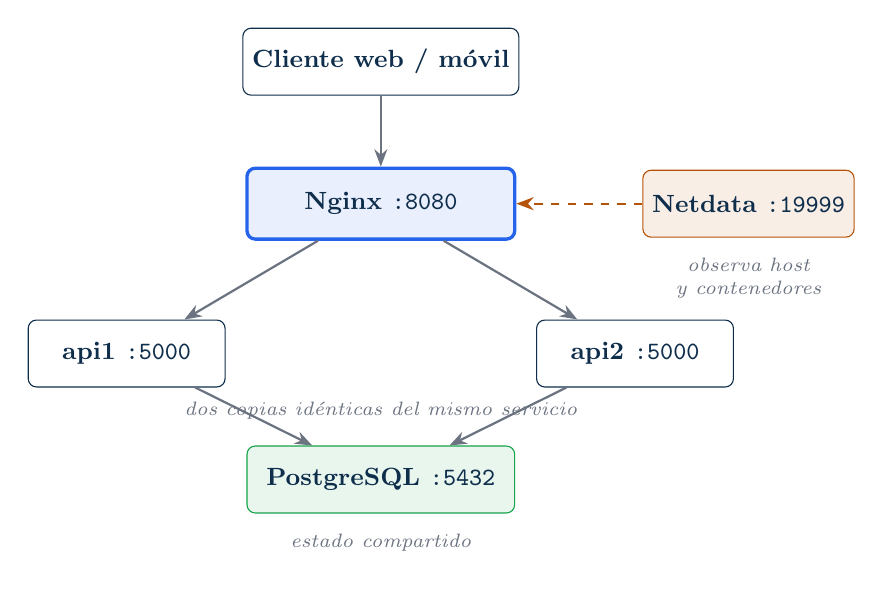
\begin{tikzpicture}[
  node distance=1.0cm and 1.4cm,
  caja/.style={draw=qcNavy, fill=white, rounded corners=3pt, minimum width=2.5cm,
               minimum height=0.85cm, font=\small\bfseries, text=qcNavy},
  lb/.style={draw=qcBlue, fill=qcBlue!10, rounded corners=3pt, minimum width=3.4cm,
             minimum height=0.9cm, font=\small\bfseries, text=qcNavy, very thick},
  db/.style={draw=qcGreen, fill=qcGreen!10, rounded corners=3pt, minimum width=3.4cm,
             minimum height=0.85cm, font=\small\bfseries, text=qcNavy},
  mon/.style={draw=qcAmber, fill=qcAmber!10, rounded corners=3pt, minimum width=2.6cm,
              minimum height=0.85cm, font=\small\bfseries, text=qcNavy},
  flecha/.style={-{Stealth[length=2.2mm]}, qcGray, thick}
]

\node[caja] (cli) {Cliente web / móvil};
\node[lb, below=0.9cm of cli] (nginx) {Nginx \texttt{:8080}};
\node[caja, below left=1.0cm and 0.25cm of nginx] (api1) {api1 \texttt{:5000}};
\node[caja, below right=1.0cm and 0.25cm of nginx] (api2) {api2 \texttt{:5000}};
\node[db, below=1.0cm of nginx, yshift=-1.6cm] (db) {PostgreSQL \texttt{:5432}};
\node[mon, right=1.6cm of nginx] (nd) {Netdata \texttt{:19999}};

\draw[flecha] (cli) -- (nginx);
\draw[flecha] (nginx) -- (api1);
\draw[flecha] (nginx) -- (api2);
\draw[flecha] (api1) -- (db);
\draw[flecha] (api2) -- (db);
\draw[qcAmber, thick, dashed, -{Stealth[length=2.2mm]}] (nd) -- (nginx);

\node[font=\scriptsize\itshape, text=qcGray] at ($(api1)!0.5!(api2) + (0,-0.72)$)
  {dos copias idénticas del mismo servicio};
\node[font=\scriptsize\itshape, text=qcGray, below=0.14cm of db] {estado compartido};
\node[font=\scriptsize\itshape, text=qcGray, below=0.14cm of nd, align=center]
  {observa host\\y contenedores};

\end{tikzpicture}
\captionof{figure}{Topología del laboratorio. El único puerto publicado hacia
fuera es el del balanceador.}
\end{center}

\begin{nota}
\textbf{El móvil no se balancea.} La app de Expo es un cliente: consume
\texttt{/api/v1}. El balanceador se coloca delante del servicio web/API para
repartir las peticiones entre dos copias idénticas del backend. Balancear
significa duplicar \emph{el mismo} servicio, no repartir componentes distintos
entre máquinas.
\end{nota}

\subsection{Por qué un laboratorio y no el entorno de producción}

La aplicación pública de QuestCash está desplegada en \textbf{Render, plan free}.
Render es un PaaS: administra el sistema operativo por nosotros. Eso tiene
consecuencias directas sobre los tres puntos de esta semana.

\begin{center}
\begin{tabular}{@{}p{4.3cm} p{5.1cm} p{5.2cm}@{}}
\toprule
\textbf{Requisito} & \textbf{En Render (free)} & \textbf{En el laboratorio} \\
\midrule
Firewall a nivel SO &
  No hay acceso al sistema operativo ni SSH. Render aplica sus propias reglas de borde. &
  \texttt{ufw} real sobre Linux, con política \emph{deny incoming}. \\[4pt]
Dos instancias &
  El plan free da una sola instancia, y además se suspende por inactividad. &
  Dos réplicas idénticas ejecutándose simultáneamente. \\[4pt]
Apagar una instancia &
  No se puede: no hay segunda instancia que apagar. &
  \texttt{docker stop qc\_api2} con tráfico en vivo. \\[4pt]
Monitoreo del sistema &
  Métricas básicas del panel de Render; sin acceso a \texttt{/proc}. &
  Netdata con visibilidad de CPU, RAM, red, disco y contenedores. \\
\bottomrule
\end{tabular}
\captionof{table}{Por qué los tres puntos requieren un entorno con control del servidor.}
\end{center}

\noindent Esto no es un rodeo: es la razón técnica por la que la práctica se
monta sobre Docker Compose. Un PaaS \emph{abstrae} justamente los mecanismos que
esta actividad pide implementar, y demostrarlos exige un entorno donde tengamos
el control.

% =====================  2. MONITOREO  =====================
\section{Monitoreo del sistema}

Se eligió \textbf{Netdata} porque muestra métricas por segundo sin configuración
previa, descubre solo los contenedores de Docker y expone un panel web listo
para capturar. Se levanta como un servicio más del stack:

\begin{lstlisting}[style=conf,language=yamlqc,caption={\texttt{docker-compose.lab.yml} — servicio de monitoreo.}]
netdata:
  image: netdata/netdata:stable
  container_name: qc_netdata
  hostname: questcash-lab
  ports:
    - "19999:19999"
  cap_add:
    - SYS_PTRACE          # leer metricas de otros procesos
    - SYS_ADMIN
  volumes:
    - /proc:/host/proc:ro             # metricas del kernel del host
    - /sys:/host/sys:ro
    - /var/run/docker.sock:/var/run/docker.sock:ro   # descubrir contenedores
\end{lstlisting}

Además, Nginx expone sus propias métricas para que Netdata las recoja
(conexiones activas, peticiones totales, peticiones en espera):

\begin{lstlisting}[style=conf,language=nginxconf,caption={\texttt{nginx.conf} — endpoint de métricas restringido a la red interna.}]
location = /nginx_status {
    stub_status;
    access_log off;
    allow 127.0.0.1;
    allow 172.16.0.0/12;    # red por defecto de Docker
    deny  all;
}
\end{lstlisting}

\subsection{Procedimiento}

\begin{enumerate}[leftmargin=1.4em,itemsep=3pt]
  \item Levantar el stack: \texttt{bash lab-semana3/scripts/00\_arrancar.sh}
  \item Generar carga real: \texttt{bash lab-semana3/scripts/03\_generar\_carga.sh}\\
        (8 clientes concurrentes durante 2 minutos contra el balanceador)
  \item Con la carga corriendo, abrir \texttt{http://localhost:19999}
  \item Capturar CPU, red, y la sección de contenedores Docker
\end{enumerate}

\begin{alerta}
\textbf{Un panel en reposo no es evidencia.} Gráficas planas demuestran que
Netdata está instalado, no que el sistema esté siendo observado bajo actividad.
Por eso las capturas se toman \emph{mientras} corre el generador de carga, y con
el selector de tiempo en «last 5 minutes» para que el pico se aprecie.
\end{alerta}

\subsection{Evidencias a incorporar}

\begin{captura}{M1}{Vista general de Netdata con CPU y red en movimiento}
\vspace{2.6cm}
\centering\itshape\color{qcGray}\footnotesize
Panel principal de \texttt{localhost:19999} durante la carga.\\
Debe verse el reloj de la barra superior para fechar la evidencia.
\vspace{2.4cm}
\end{captura}

\vspace{0.6em}
\begin{captura}{M2}{System overview → CPU: el pico coincidiendo con la ráfaga}
\vspace{2.2cm}
\centering\itshape\color{qcGray}\footnotesize
Gráfica de utilización de CPU con el escalón provocado por los 8 clientes.
\vspace{2.0cm}
\end{captura}

\vspace{0.6em}
\begin{captura}{M3}{Docker containers: los 5 contenedores con su consumo}
\vspace{2.2cm}
\centering\itshape\color{qcGray}\footnotesize
Debe listar \texttt{qc\_lb}, \texttt{qc\_api1}, \texttt{qc\_api2},
\texttt{qc\_db} y \texttt{qc\_netdata}.
\vspace{2.0cm}
\end{captura}

\vspace{0.8em}
\noindent El script \texttt{03\_generar\_carga.sh} complementa las capturas con
métricas en texto: peticiones totales, \emph{throughput} en req/s, la salida de
\texttt{stub\_status} y el consumo por contenedor según \texttt{docker stats}.
Ese archivo (\texttt{evidencia/03\_carga.txt}) sirve como respaldo numérico de lo
que muestran las gráficas.

% =====================  3. FIREWALL  =====================
\section{Firewall a nivel de sistema operativo}

\subsection{Política}

El firewall aplica el principio de mínimo privilegio a la red: \textbf{se
deniega todo lo entrante} y se abre únicamente lo que el servicio necesita.

\begin{center}
\begin{tabular}{@{}l l p{8.4cm}@{}}
\toprule
\textbf{Dirección} & \textbf{Política} & \textbf{Razón} \\
\midrule
Entrante  & \http{qcRed}{DENY}    & Nada entra salvo lo explícitamente permitido. Cada puerto abierto es una puerta más que alguien puede tocar. \\[3pt]
Saliente  & \http{qcGreen}{ALLOW} & El servidor necesita salir: actualizaciones del SO, DNS, renovación de certificados, APIs externas. \\
\bottomrule
\end{tabular}
\captionof{table}{Política por defecto de \texttt{ufw}.}
\end{center}

\subsection{Puertos abiertos y por qué}

\begin{center}
\begin{tabular}{@{}c l l p{7.6cm}@{}}
\toprule
\textbf{Puerto} & \textbf{Proto} & \textbf{Servicio} & \textbf{Justificación} \\
\midrule
22  & TCP & SSH   & Única vía de administración. Se abre con \texttt{ufw limit}, que bloquea una IP tras 6 intentos en 30\,s: frena la fuerza bruta automatizada. \\[4pt]
80  & TCP & HTTP  & Necesario para el reto HTTP-01 de Let's Encrypt y para redirigir a HTTPS. No sirve contenido real. \\[4pt]
443 & TCP & HTTPS & Por aquí entra \textbf{todo} el tráfico de usuarios. Es el único puerto que la aplicación realmente necesita. \\
\bottomrule
\end{tabular}
\captionof{table}{Puertos permitidos.}
\end{center}

\subsection{Puertos deliberadamente cerrados}

Documentar lo que se cierra es tan importante como documentar lo que se abre:
demuestra que la decisión fue consciente y no un descuido.

\begin{center}
\begin{tabular}{@{}c l p{9.6cm}@{}}
\toprule
\textbf{Puerto} & \textbf{Servicio} & \textbf{Por qué NO se abre} \\
\midrule
5432  & PostgreSQL      & Solo alcanzable desde la red interna de Docker. Una base de datos expuesta a internet es una de las causas más comunes de fuga de datos y ransomware. \\[4pt]
5000  & Flask/Gunicorn  & Las instancias solo hablan con Nginx. Si fueran accesibles directo, se podría saltar el balanceador, el TLS y cualquier límite de tasa. \\[4pt]
8080  & Nginx del lab   & Puerto de desarrollo. En un servidor real el proxy escucha en 80 y 443. \\[4pt]
19999 & Netdata         & El panel expone topología, procesos y métricas: es reconocimiento gratis para un atacante. Se accede por túnel SSH. \\
\bottomrule
\end{tabular}
\captionof{table}{Puertos cerrados y su razón.}
\end{center}

\begin{nota}
Para llegar a Netdata sin exponerlo:
\texttt{ssh -L 19999:localhost:19999 usuario@servidor} y luego abrir
\texttt{http://localhost:19999} en la máquina local. El puerto nunca queda
publicado a internet.
\end{nota}

\subsection{Aplicación de las reglas}

\begin{lstlisting}[style=conf,caption={\texttt{lab-semana3/firewall/ufw\_reglas.sh} — extracto.}]
# Politica por defecto
sudo ufw default deny incoming
sudo ufw default allow outgoing

# SSH con limite de tasa contra fuerza bruta
sudo ufw limit 22/tcp  comment 'SSH - administracion remota (rate limited)'

# HTTP solo para redireccion y reto ACME
sudo ufw allow 80/tcp  comment 'HTTP - redireccion a HTTPS y reto ACME'

# HTTPS: el trafico real de la aplicacion
sudo ufw allow 443/tcp comment 'HTTPS - trafico de la aplicacion'

sudo ufw --force enable
sudo ufw status verbose
\end{lstlisting}

\begin{alerta}
\textbf{Advertencia importante sobre el entorno.} \texttt{ufw} es un envoltorio
de \texttt{iptables}, que pertenece al kernel de \textbf{Linux}. macOS usa
\texttt{pf}, que es otra cosa, y Docker Desktop ejecuta los contenedores dentro
de su propia máquina virtual gestionando sus reglas de red automáticamente. Por
lo tanto \textbf{este punto no se puede demostrar sobre macOS}.

Para presentar evidencia real hay dos caminos válidos: (a) una \textbf{VM Ubuntu
en VirtualBox}, donde se ejecuta el script y se captura la salida; o (b) un
\textbf{VPS} con IP pública, que permite además verificar desde fuera con
\texttt{nmap} que solo responden 22, 80 y 443. La opción (b) es la más
contundente porque demuestra el firewall desde la perspectiva de un atacante y
no solo desde la configuración declarada.
\end{alerta}

\subsection{Evidencias a incorporar}

\begin{captura}{F1}{\texttt{sudo ufw status verbose} — política y reglas activas}
\vspace{2.4cm}
\centering\itshape\color{qcGray}\footnotesize
Debe verse \texttt{Status: active}, la línea\\
\texttt{Default: deny (incoming), allow (outgoing)} y las tres reglas.
\vspace{2.2cm}
\end{captura}

\vspace{0.6em}
\begin{captura}{F2}{\texttt{sudo ss -tulnp | grep LISTEN} — qué escucha realmente}
\vspace{2.0cm}
\centering\itshape\color{qcGray}\footnotesize
Contrasta la configuración declarada con los procesos que de hecho\\
tienen un socket abierto.
\vspace{1.8cm}
\end{captura}

\vspace{0.6em}
\begin{captura}{F3}{\texttt{nmap} desde otra máquina — la vista del atacante}
\vspace{2.0cm}
\centering\itshape\color{qcGray}\footnotesize
El escaneo solo debe encontrar 22, 80 y 443 abiertos.\\
\emph{Opcional: requiere IP alcanzable desde otro equipo.}
\vspace{1.8cm}
\end{captura}

% =====================  4. BALANCEADOR  =====================
\section{Balanceador de carga con Nginx}

Nginx funciona como \emph{reverse proxy} y balanceador: el cliente se conecta a
Nginx y este distribuye las peticiones entre dos instancias equivalentes de
QuestCash. Ambas usan la misma imagen, la misma configuración y la misma base de
datos.

\subsection{El grupo de servidores}

\begin{lstlisting}[style=conf,language=nginxconf,caption={\texttt{nginx.conf} — definición del \emph{upstream}.}]
upstream questcash_api {
    server api1:5000 max_fails=1 fail_timeout=5s;
    server api2:5000 max_fails=1 fail_timeout=5s;

    keepalive 32;           # conexiones reutilizadas hacia el backend
}
\end{lstlisting}

\noindent Tres decisiones vale la pena explicar:

\begin{itemize}[leftmargin=1.4em,itemsep=4pt]
  \item \textbf{Round-robin} (el algoritmo por defecto): Nginx alterna entre los
        servidores de la lista. Se espera un reparto cercano al 50/50, que es
        justamente lo que mide la prueba 1.
  \item \textbf{\texttt{max\_fails=1 fail\_timeout=5s}}: al primer fallo, Nginx
        marca la instancia como caída y deja de mandarle tráfico durante 5
        segundos; después la vuelve a probar sola. Este es el \emph{health check
        pasivo}. Nginx de código abierto no hace sondeos activos —eso es Nginx
        Plus—, así que la detección ocurre al intentar usar el servidor.
  \item \textbf{\texttt{keepalive 32}}: mantiene conexiones abiertas hacia los
        backends en lugar de renegociar TCP en cada petición.
\end{itemize}

\subsection{El reparto y la tolerancia a fallas}

\begin{lstlisting}[style=conf,language=nginxconf,caption={\texttt{nginx.conf} — bloque \texttt{location} principal.}]
location / {
    proxy_pass http://questcash_api;

    proxy_http_version 1.1;
    proxy_set_header Connection "";
    proxy_set_header Host              $host;
    proxy_set_header X-Real-IP         $remote_addr;
    proxy_set_header X-Forwarded-For   $proxy_add_x_forwarded_for;
    proxy_set_header X-Forwarded-Proto $scheme;

    # Si la instancia elegida no responde, Nginx REINTENTA en la otra
    # dentro de la MISMA peticion: el cliente nunca ve el error.
    proxy_next_upstream       error timeout http_502 http_503 http_504;
    proxy_next_upstream_tries 2;

    proxy_connect_timeout 2s;
}
\end{lstlisting}

\begin{nota}
\texttt{proxy\_next\_upstream} es la pieza que convierte «dos servidores» en
«alta disponibilidad». Sin ella, las peticiones que caigan en la instancia
apagada devolverían \http{qcRed}{502} hasta que Nginx la marque como caída. Con
ella, el reintento ocurre dentro de la misma petición y el resultado esperado de
la prueba de failover es \textbf{100\,\% de disponibilidad}, no «unos cuantos
errores al principio».
\end{nota}

\subsection{Cómo se sabe qué instancia respondió}

Para poder \emph{medir} el reparto, Nginx etiqueta cada respuesta y cada línea
de su log con la instancia que la atendió:

\begin{lstlisting}[style=conf,language=nginxconf,caption={\texttt{nginx.conf} — instrumentación para la evidencia.}]
log_format lb '$remote_addr [$time_local] "$request" '
              'status=$status upstream=$upstream_addr '
              'upstream_status=$upstream_status '
              'rt=$request_time urt=$upstream_response_time';

# Cabecera de diagnostico (en produccion se quita: revela la topologia)
add_header X-Served-By $upstream_addr always;
\end{lstlisting}

\subsection{Aislamiento de las instancias}

En \texttt{docker-compose.lab.yml}, \textbf{solo el balanceador publica un
puerto}. \texttt{api1} y \texttt{api2} no tienen sección \texttt{ports:}, así
que son inalcanzables desde fuera de la red de Docker:

\begin{lstlisting}[style=conf,language=yamlqc,caption={\texttt{docker-compose.lab.yml} — extracto de las instancias y el proxy.}]
api1:
  build: { context: ., dockerfile: Dockerfile }
  container_name: qc_api1
  command: gunicorn --bind 0.0.0.0:5000 --workers 2 app:app
  environment:
    DATABASE_URL: postgresql://questcash:PURGADO-ROTAR-EN-RENDER@db:5432/questcash
    INSTANCE_ID: api1
  depends_on:
    db: { condition: service_healthy }
  # Sin `ports:` a proposito -> no accesible desde fuera

lb:
  image: nginx:1.27-alpine
  container_name: qc_lb
  ports:
    - "8080:80"          # en produccion seria 80:80 y 443:443
  volumes:
    - ./lab-semana3/nginx/nginx.conf:/etc/nginx/nginx.conf:ro
  depends_on: [api1, api2]
\end{lstlisting}

\begin{nota}
Se usa \textbf{Gunicorn} y no el servidor de desarrollo de Flask. El de Flask es
monoproceso y no está pensado para concurrencia: con 8 clientes simultáneos los
resultados de la prueba de carga no medirían el balanceo, medirían el cuello de
botella del servidor de desarrollo.
\end{nota}

\subsection{Evidencias a incorporar}

\begin{captura}{B1}{\texttt{docker compose ps} — los 5 contenedores en \texttt{Up}}
\vspace{2.0cm}
\centering\itshape\color{qcGray}\footnotesize
Estado inicial: \texttt{qc\_lb}, \texttt{qc\_api1}, \texttt{qc\_api2},
\texttt{qc\_db}, \texttt{qc\_netdata}.
\vspace{1.8cm}
\end{captura}

\vspace{0.6em}
\begin{captura}{B2}{Salida de \texttt{01\_reparto.sh} — distribución del tráfico}
\vspace{2.2cm}
\centering\itshape\color{qcGray}\footnotesize
Conteo de peticiones por instancia sobre 200 peticiones.\\
Se espera un reparto cercano al 50/50 y 0 errores.
\vspace{2.0cm}
\end{captura}

% =====================  5. FAILOVER  =====================
\section{Prueba de tolerancia a fallas}

Esta es la evidencia central del entregable. El script
\texttt{02\_failover.sh} automatiza la prueba completa para que el resultado sea
medible y no una impresión:

\begin{enumerate}[leftmargin=1.4em,itemsep=3pt]
  \item Lanza una ráfaga continua de peticiones al balanceador (una cada 0.5\,s
        durante 45\,s), registrando hora, código HTTP e instancia que respondió.
  \item A los 15\,s \textbf{apaga \texttt{qc\_api2}} con el tráfico corriendo.
  \item A los 30\,s la vuelve a encender.
  \item Al terminar, calcula disponibilidad, peticiones fallidas y reparto por
        instancia, y muestra cómo lo registró Nginx en su log de error.
\end{enumerate}

\begin{lstlisting}[style=conf,caption={\texttt{02\_failover.sh} — núcleo de la prueba.}]
# Racha de peticiones en segundo plano
(
  fin=$(( $(date +%s) + DURACION ))
  while [ "$(date +%s)" -lt "$fin" ]; do
    code=$(curl -s -m 5 -o /dev/null -D /tmp/qc_h2.txt \
                -w "%{http_code}" "$BASE$RUTA")
    inst=$(awk 'tolower($1)=="x-served-by:" {print $2}' /tmp/qc_h2.txt)
    printf "%s  HTTP=%s  instancia=%s\n" "$(date +%H:%M:%S)" "$code" "$inst" >> "$LOG"
    sleep 0.5
  done
) &

sleep $(( DURACION / 3 ))
docker stop "$VICTIMA"      # <-- se apaga una instancia EN VIVO
sleep $(( DURACION / 3 ))
docker start "$VICTIMA"     # <-- y se comprueba que Nginx la reincorpora
\end{lstlisting}

\subsection{Qué se debe observar}

\begin{center}
\begin{tabular}{@{}l p{10.4cm}@{}}
\toprule
\textbf{Métrica} & \textbf{Resultado esperado y por qué} \\
\midrule
Disponibilidad      & \textbf{100\,\%}. Gracias a \texttt{proxy\_next\_upstream}, las peticiones que tocan la instancia caída se reintentan en la otra dentro de la misma petición. \\[4pt]
Peticiones fallidas & \textbf{0}. Si aparecen 502 o timeouts, revisar que \texttt{proxy\_next\_upstream} esté activo. \\[4pt]
Reparto             & $\approx$50/50 antes del apagón, \textbf{100\,\% en la sobreviviente} durante la caída, y vuelta al reparto tras reencender. \\[4pt]
Log de error Nginx  & Debe aparecer un mensaje de conexión rechazada hacia \texttt{api2}: es la prueba de que Nginx \emph{detectó} la falla, no de que algo salió mal. \\
\bottomrule
\end{tabular}
\captionof{table}{Criterios de aceptación de la prueba de failover.}
\end{center}

\begin{nota}
\textbf{Interpretación técnica.} Balancear no consiste en apagar frontend, API y
base de datos entre sí —eso rompe el sistema y es el resultado esperado, no una
prueba. La prueba correcta consiste en apagar \textbf{una copia del mismo
servicio} que está detrás de Nginx. La otra copia permanece disponible y sigue
accediendo al mismo PostgreSQL, que es lo que hace que el usuario no note nada.
\end{nota}

\subsection{Evidencias a incorporar}

\begin{captura}{B3}{Línea de tiempo del failover con la instancia ya detenida}
\vspace{2.6cm}
\centering\itshape\color{qcGray}\footnotesize
Debe verse la marca \texttt{>>> APAGANDO qc\_api2} y, en las líneas\\
siguientes, \texttt{HTTP=200} atendido íntegramente por \texttt{qc\_api1}.
\vspace{2.4cm}
\end{captura}

\vspace{0.6em}
\begin{captura}{B4}{Navegador cargando el sitio con una instancia caída}
\vspace{2.4cm}
\centering\itshape\color{qcGray}\footnotesize
\texttt{http://localhost:8080/login} respondiendo, junto a una terminal\\
con \texttt{docker compose ps} mostrando \texttt{qc\_api2} en \texttt{Exited}.
\vspace{2.2cm}
\end{captura}

\vspace{0.6em}
\begin{captura}{B5}{Resumen final: disponibilidad y peticiones fallidas}
\vspace{2.2cm}
\centering\itshape\color{qcGray}\footnotesize
El bloque RESUMEN del script, con la disponibilidad calculada.
\vspace{2.0cm}
\end{captura}

\begin{nota}
\textbf{Alternativa recomendada: video de 60 segundos.} El entregable acepta
video, y para esta prueba es más convincente que las capturas porque muestra la
continuidad. Basta grabar con \texttt{Cmd + Shift + 5} tres elementos visibles a
la vez: la terminal corriendo el script, el navegador recargando el sitio, y otra
terminal con \texttt{docker compose ps}.
\end{nota}

% =====================  6. PROCEDIMIENTO  =====================
\section{Procedimiento de implementación}

Todo el laboratorio vive en \texttt{questcash\_web/lab-semana3/} y se ejecuta
desde la raíz del proyecto.

\begin{consola}[title={Levantar el laboratorio y correr las pruebas}]
\begin{lstlisting}[style=terminal]
cd ~/questcash_web

# 1) Construir y levantar: Nginx + 2 instancias + Postgres + Netdata
bash lab-semana3/scripts/00_arrancar.sh

# 2) Comprobar que el trafico se reparte entre las dos instancias
bash lab-semana3/scripts/01_reparto.sh

# 3) PRUEBA CENTRAL: apagar una instancia con trafico en vivo
bash lab-semana3/scripts/02_failover.sh

# 4) Generar carga y capturar el monitoreo (abrir localhost:19999)
bash lab-semana3/scripts/03_generar_carga.sh

# Bajar todo al terminar
docker compose -f docker-compose.lab.yml down -v
\end{lstlisting}
\end{consola}

\vspace{0.5em}
\begin{consola}[title={Firewall — ejecutar en una VM Ubuntu o VPS, no en macOS}]
\begin{lstlisting}[style=terminal]
sudo bash lab-semana3/firewall/ufw_reglas.sh

# Comprobaciones que valen como evidencia
sudo ufw status verbose
sudo ufw status numbered
sudo ss -tulnp | grep LISTEN
nmap -Pn <ip-del-servidor>        # desde OTRA maquina
\end{lstlisting}
\end{consola}

\subsection{Estructura de archivos entregada}

\begin{lstlisting}[style=terminal]
questcash_web/
  docker-compose.lab.yml          <- stack completo del laboratorio
  lab-semana3/
    README.md                     <- guia de uso
    CAPTURAS.md                   <- que capturar y cuando
    nginx/nginx.conf              <- balanceador (upstream + failover)
    scripts/00_arrancar.sh        <- levanta y verifica el stack
    scripts/01_reparto.sh         <- mide la distribucion del trafico
    scripts/02_failover.sh        <- prueba de tolerancia a fallas
    scripts/03_generar_carga.sh   <- carga sostenida para el monitoreo
    firewall/ufw_reglas.sh        <- reglas comentadas
    firewall/README-firewall.md   <- justificacion puerto por puerto
    evidencia/                    <- salidas en texto de cada prueba
\end{lstlisting}

\begin{nota}
El script de arranque incluye un guardarraíl: si \texttt{.dockerignore} no
excluye \texttt{data/raw/}, lo agrega. Esa carpeta contiene unos 750\,MB de CSVs
del ENIGH que la aplicación no usa en tiempo de ejecución —solo consume
\texttt{data/processed/}— y sin excluirla Docker los copiaría al contexto de
construcción en cada \emph{build}.
\end{nota}

% =====================  7. EVIDENCIAS  =====================
\section{Estado de las evidencias de la entrega}

\begin{center}
\begin{tabular}{@{}p{3.9cm} p{5.4cm} c p{2.9cm}@{}}
\toprule
\textbf{Evidencia} & \textbf{Qué debe mostrar} & \textbf{Estado} & \textbf{Dónde} \\
\midrule
Configuración del balanceador & \texttt{upstream} con 2 servidores, round-robin, \texttt{proxy\_next\_upstream} & \ok & Anexo A \\[4pt]
Definición de las 2 instancias & \texttt{api1} y \texttt{api2} sin puertos publicados & \ok & Anexo B \\[4pt]
Reglas de firewall documentadas & Puertos abiertos, cerrados y su justificación & \ok & Sección 3, Anexo C \\[4pt]
Monitoreo con actividad real & Netdata bajo carga: CPU, red, contenedores & \pend & Capturas M1--M3 \\[4pt]
\texttt{ufw} aplicado & \texttt{ufw status verbose} en Linux & \pend & Capturas F1--F3 \\[4pt]
Reparto de carga medido & Distribución sobre 200 peticiones & \pend & Captura B2 \\[4pt]
Prueba de failover & Instancia apagada y sitio respondiendo & \pend & Capturas B3--B5 o video \\
\bottomrule
\end{tabular}
\captionof{table}{Qué está listo y qué falta ejecutar.}
\end{center}

\begin{alerta}
\textbf{Nota de integridad académica.} Este documento no incluye capturas
simuladas. Las configuraciones son archivos reales y ejecutables del proyecto;
las evidencias visuales aparecen como recuadros vacíos hasta ser sustituidas por
capturas obtenidas durante la ejecución real. Presentar un \emph{mockup} como
captura sería, además de deshonesto, inútil: no demuestra que el sistema
funcione.
\end{alerta}

% =====================  8. CONCLUSIÓN  =====================
\section{Conclusión}

\begin{enumerate}[leftmargin=1.4em,itemsep=4pt]
  \item \textbf{Los tres mecanismos son complementarios, no independientes.} El
        monitoreo permite \emph{observar} el estado del sistema; el firewall
        \emph{reduce} la superficie de ataque; el balanceo \emph{mantiene} la
        disponibilidad cuando una instancia falla. Ninguno sustituye a los otros.
  \item \textbf{La arquitectura separa el punto de entrada público de las
        instancias internas.} Solo el balanceador publica un puerto; las
        instancias y PostgreSQL viven en la red interna de Docker. Esa
        separación es una medida de seguridad por sí misma, independiente del
        firewall del sistema operativo.
  \item \textbf{La prueba de apagar una instancia es la evidencia principal de
        tolerancia a fallas}, y está automatizada para producir un número —la
        disponibilidad durante la caída— en lugar de una impresión.
  \item \textbf{El entorno de producción impone límites reales.} Render en plan
        free no permite firewall a nivel SO, ni SSH, ni una segunda instancia.
        Reconocerlo y montar el laboratorio es la respuesta técnicamente
        correcta, no un atajo.
\end{enumerate}

\vspace{0.8em}
\begin{nota}
\textbf{Siguiente paso natural.} El laboratorio deja el balanceador escuchando en
HTTP. El cierre lógico de esta línea de trabajo —y el pendiente que quedó
señalado en el reporte de la semana 2— es terminar TLS en el propio Nginx:
certificado de Let's Encrypt, redirección de 80 a 443 y cabecera HSTS. Con eso,
el puerto 443 del firewall deja de ser una regla declarada y pasa a ser el
camino real del tráfico.
\end{nota}

% =====================  ANEXOS  =====================
\newpage
\section*{Anexo A — \texttt{nginx.conf} completo}
\addcontentsline{toc}{section}{Anexo A}

\lstinputlisting[style=conf,language=nginxconf]{../../lab-semana3/nginx/nginx.conf}

\newpage
\section*{Anexo B — \texttt{docker-compose.lab.yml} completo}
\addcontentsline{toc}{section}{Anexo B}

\lstinputlisting[style=conf,language=yamlqc]{../../lab-semana3/docker-compose.lab.yml}

\newpage
\section*{Anexo C — \texttt{ufw\_reglas.sh} completo}
\addcontentsline{toc}{section}{Anexo C}

\lstinputlisting[style=conf]{../../lab-semana3/firewall/ufw_reglas.sh}

\vspace{1.2em}
\noindent\textbf{Fuentes de trabajo}

\begin{itemize}[leftmargin=1.4em,itemsep=2pt]
  \item Repositorio web/backend: \texttt{questcash\_web} — Flask, API \texttt{/api/v1}, PostgreSQL.
  \item Repositorio móvil: \texttt{questcash\_mobile} — Expo / React Native, cliente de la API.
  \item Reporte de la semana 2: \texttt{docs/semana2/reporte\_semana2.tex} — autenticación JWT.
  \item Actividad académica: EP.03.01 — Monitoreo, firewall y balanceador de carga.
\end{itemize}

\end{document}
